\section{Preliminaries}\label{sec:preliminaries}

In this section, we introduce the mathematical formulation of flow matching and describe how the denoising process can be mapped as a multi-step MDP.


\paragraph{Flow Matching.}\label{subsec:flow_matching}
Let \(\vx_0 \sim X_0\) be a data sample from the true distribution, and \(\vx_1 \sim X_1\) denote a noise sample. Recent advanced image-generation models (e.g., \cite{sd3,flux2024}) and video-generation models (e.g., \cite{kling,sora,wanx,hunyuanvideo}) adopt the Rectified Flow~\cite{rectified_flow} framework, which defines the “noised” data \(\vx_t\) as
\begin{equation}
\label{eq:flow_forward}
    \vx_t = (1-t)\,\vx_0 \;+\; t\,\vx_1,
\end{equation}
for \(t \in [0,1]\). Then a transformer model are trained to directly regress the velocity field \(\vv_\theta(\vx_t, t)\) by minimizing the Flow Matching objective \cite{lipman2022flow,rectified_flow}:
\begin{equation}
\label{eq:flow_loss}
    \loss(\theta) = \mathbb{E}_{t,\;\vx_0\sim X_0,\;\vx_1 \sim X_1} 
    \bigl[\;\|\vv \;-\; \vv_\theta(\vx_t,t)\|^2\bigr],
\end{equation}
where the target velocity field is \(\vv = \vx_1 - \vx_0\).

% The alignment of language models is typically cast as a KL-constrained optimization problem~\citep{ziegler2019fine}:
% \begin{subequations}
% \label{eq:obj}
% \begin{align}
%     \argmax_{\pi} \quad & \mathbb{E}_{\rvx \sim p(\rvx), \rvy \sim \pi(\rvy \mid \rvx)}\left[r(\rvx, \rvy)\right] \\
%     \text{s.t.} \quad & \mathbb{E}_{\rvx \sim p(\rvx)} \left[\mathbb{D}_{\mathrm{KL}}\left(\pi(\rvy \mid \rvx) \,\|\, \pi_{\mathrm{ref}}(\rvy \mid \rvx)\right)\right] \leq \epsilon,
% \end{align}
% \end{subequations}
% where $p(\rvx)$ is a distribution of prompts, $\rvy$ is the complete language model response, $r$ is a preference reward function that encourages human-preferred responses, and $\mathbb{D}_{\mathrm{KL}}$ limits how far the optimized language model $\pi$ can deviate from the reference (untuned) model $\pi_{\text{ref}}$.
% There are two main categories of alignment algorithms: (1) \textit{search-based} algorithms that optimize Eq.~\ref{eq:obj} with graph-based search during inference
% ~\citep{gao2023scaling, mudgal2023controlled, liu2023making, feng2023alphazero, mitchell2023emulator, liu2024tuning}, and (2) \textit{learning-based} algorithms that optimize Eq.~\ref{eq:obj} through gradient descent, aiming for a parametrized optimal language model~\citep{ziegler2019fine, zhao2023slic, rafailov2024direct, ethayarajh2024kto}. 
% Our work falls in the first category, proposing a search-based algorithm capable of using small language models to guide the decoding of a large language model to align with human preferences. 
% \footnote{For search-based algorithms, it is the response $\rvy$ that is searched rather than the language model $\pi$, therefore $\argmax_{\rvy}$ should be more appropriate. However, for brevity, we unify searching and learning in a unified framework ($\argmax_{\pi}$) by interpreting the searched responses as equivalently sampled from a latent model.}


\begin{figure}[t]
\centering
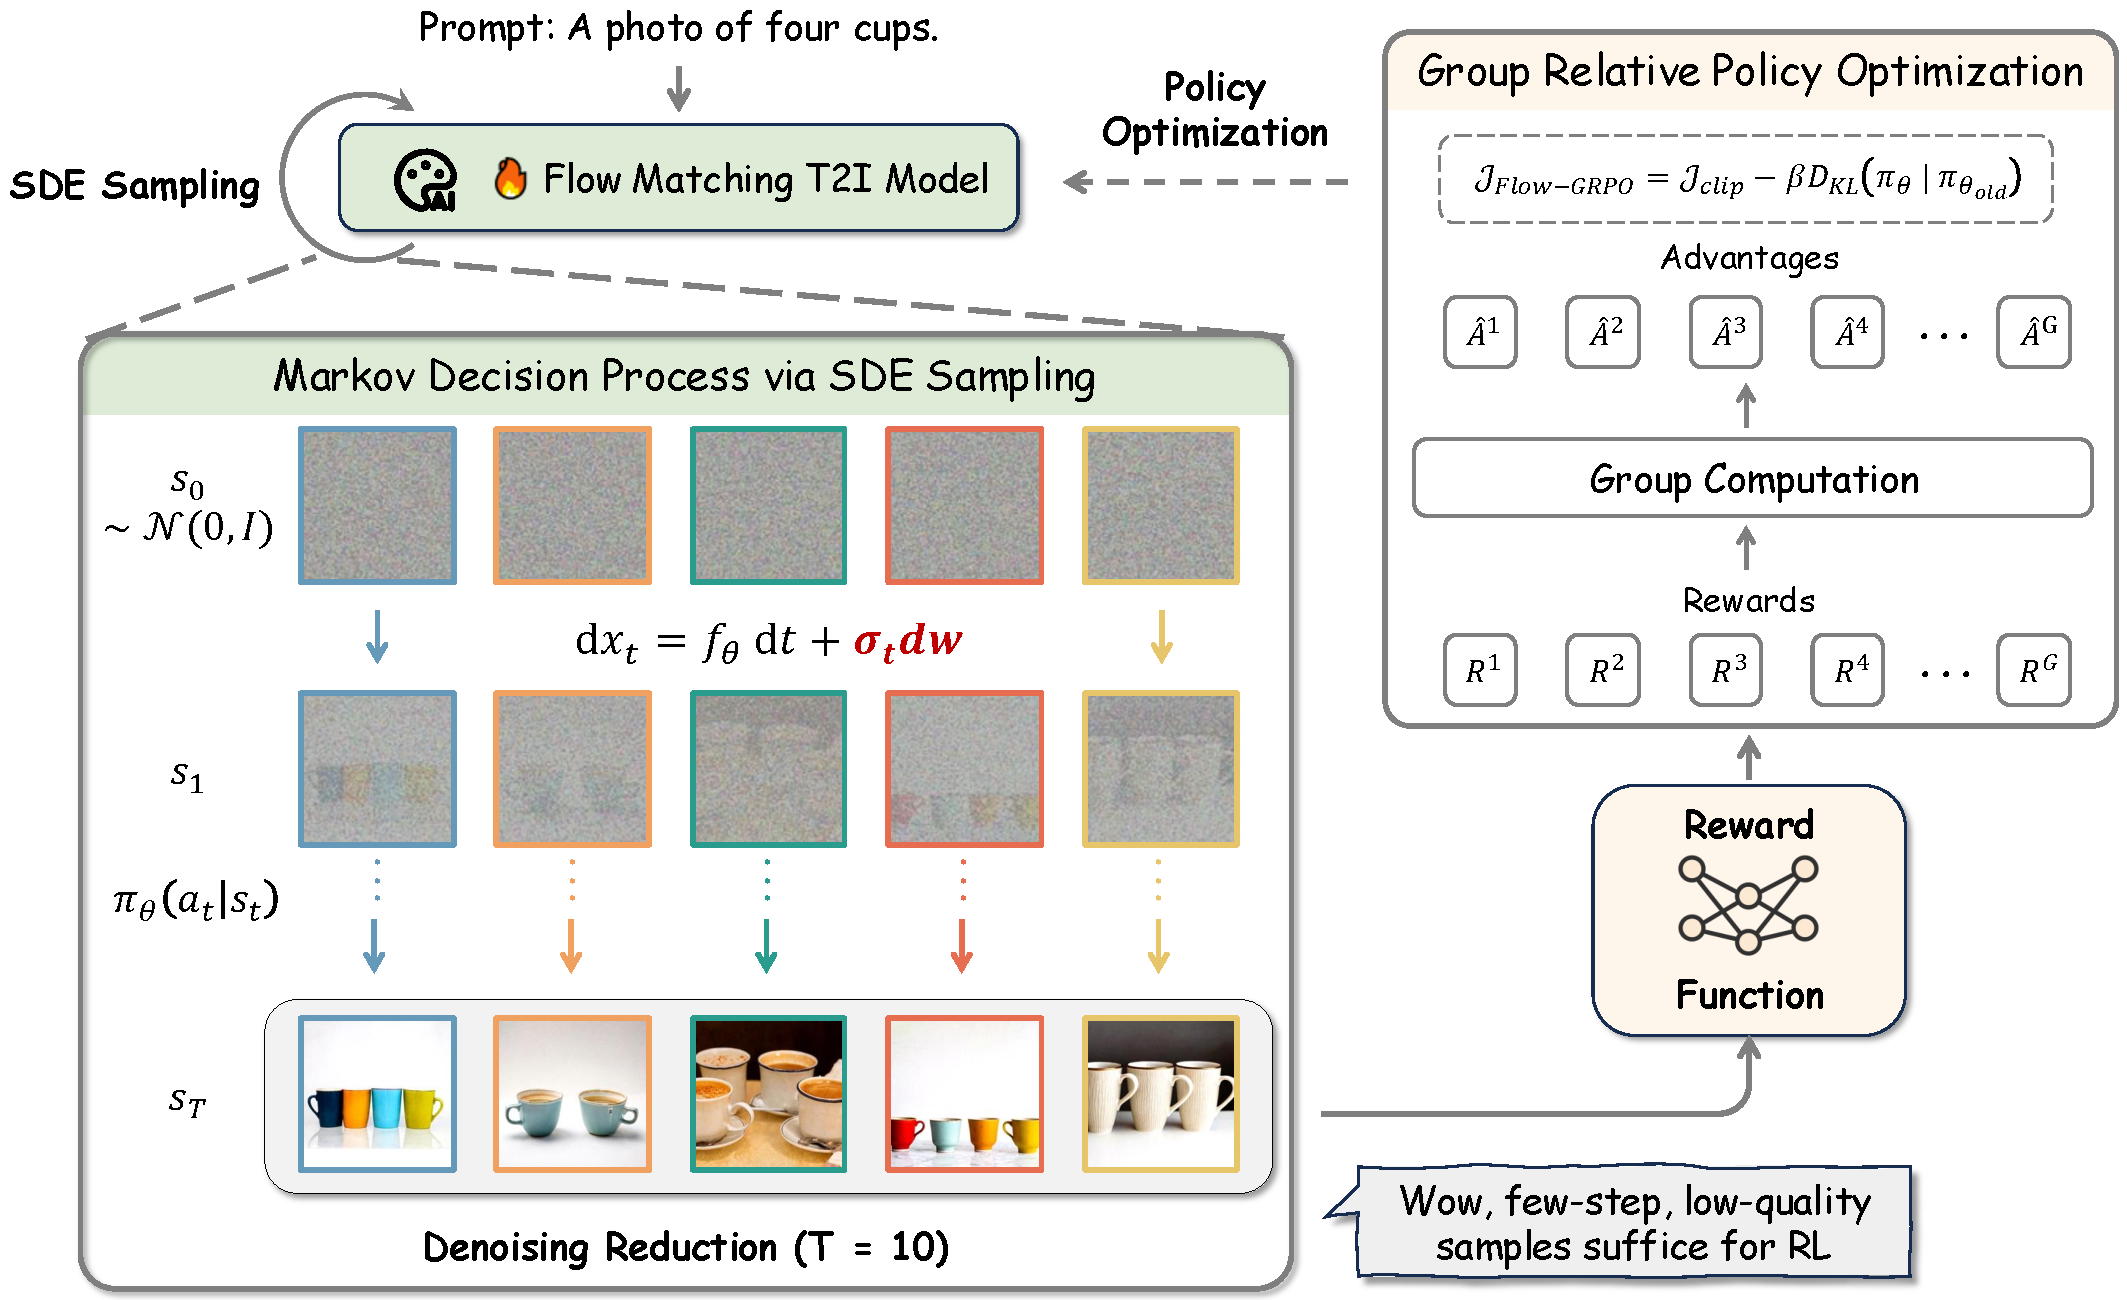
\includegraphics[width=0.9\textwidth]{src/method.pdf}
% \caption{Overview of Flow-GRPO. Given an input prompt, we first introduce the ODE-to-SDE strategy to implement stochastic sampling for online RL. Meanwhile, during the denoising process, we utilize the Denoising Reduction strategy to reduce the denoising steps in training to improve the sampling efficiency. Finally, we apply the GRPO strategy to perform the policy optimization and obtain the final aligned models.
% }
% \caption{Flow-GRPO processes an input prompt in three stages. First, an ODE-to-SDE strategy enables stochastic sampling for online RL. Second, a Denoising Reduction strategy reduces denoising steps during training to improve sampling efficiency. Finally, the GRPO strategy optimizes the policy to produce the aligned models.}
\caption{\textbf{Overview of Flow-GRPO.} 
Given a prompt set, we introduce an ODE-to-SDE strategy to enable stochastic sampling for online RL.
With Denoising Reduction (only T = 10 steps), we efficiently gather low-quality but still informative trajectories.
Rewards from these trajectories feed the GRPO loss, which updates the model online and yields an aligned policy.}
\vspace{-2mm}
\label{fig:method}
\end{figure}

\paragraph{Denoising as an MDP.}\label{subsec:denoising_as_mdp}
As shown in~\citep{ddpo}, the iterative denoising process in flow matching models can be formulated as a Markov Decision Process (MDP) \((\mathcal{S}, \mathcal{A}, \rho_0, P, R)\). The state at step \(t\) is \(\vs_t \triangleq (\vc, t, \vx_t)\), the action is the denoised sample \(\va_t \triangleq \vx_{t-1}\) predicted by the model, and the policy is \(\pi(\va_t \mid \vs_t) \triangleq p_\theta(\vx_{t-1} \mid \vx_t, \vc)\). 
The transition is deterministic: \(P(\vs_{t+1} \mid \vs_t, \va_t) \triangleq (\delta_\vc, \delta_{t-1}, \delta_{\vx_{t-1}})\), and the initial state distribution is \(\rho_0(\vs_0) \triangleq (p(\vc), \delta_T, \mathcal{N}(\mathbf{0}, \mathbf{I}))\), where \(\delta_y\) is the Dirac delta distribution centered at \(y\). 
The reward is only given at the final step: \(R(\vs_t, \va_t) \triangleq r(\vx_0, \vc)\) if \(t = 0\), and 0 otherwise.


% \begin{equation}
% \begin{aligned}
% \mathcal{J}_\text{GRPO}(\theta)& = \mathbb{E}_{(q,a)\sim \mathcal{D}, \{o_i\}_{i=1}^G\sim \pi_{\theta_\text{old}}(\cdot\mid q)} \\&
% \Bigg[ \frac{1}{G}\sum_{i=1}^{G} \frac{1}{|o_i|}\sum_{t=1}^{|o_i|} \Bigg( 
% \min \Big( r_{i,t}(\theta) \hat{A}_{i,t},  
% \ \text{clip} \Big( r_{i,t}(\theta), 1 - \varepsilon, 1 + \varepsilon \Big) \hat{A}_{i,t} \Big)
% - \beta D_{\text{KL}}(\pi_{\theta} || \pi_{\text{ref}}) 
% \Bigg) \Bigg],
% \label{eq:grpoloss}
% \end{aligned}
% \end{equation}
% where
% \begin{equation}
%     r_{i,t}(\theta)=\frac{\pi_{\theta}(o_{i,t} \mid q, o_{i,<t})}{\pi_{\theta_{\text{old}}}(o_{i,t} \mid q,o_{i,<t})}.
% \end{equation}

% The analytical solution to Eq.~\ref{eq:obj} can be obtained through the following Lagrangian~\citep{peng2019advantage, nair2020awac}:
% \begin{equation}\label{eq:lg-obj}
%     \mathcal{L(\pi, \beta)} = \mathbb{E}_{\rvx \sim p(\rvx), \rvy \sim \pi(\rvy \mid \rvx)}\left[r(\rvx, \rvy) + \beta\left(\epsilon - \mathbb{D}_{\mathrm{KL}}\left(\pi(\rvy \mid \rvx) \,\|\, \pi_{\mathrm{ref}}(\rvy \mid \rvx)\right)\right) \right],
% \end{equation}
% which has a well-known closed-form solution that expresses a duality between the reward function $r(\rvx, \rvy)$ and the optimal language model $\pi^*(\rvy \mid \rvx)$~\citep{ziebart2008maximum, levine2018reinforcement}:
% \begin{equation}\label{eq:duality}
%     r(\rvx, \rvy) = \beta \log \frac{\pi^*(\rvy \mid \rvx)}{\pi_{\text{ref}}(\rvy \mid \rvx)} + \beta \log Z(\rvx),
% \end{equation}
% where $Z(\rvx) = \sum_\rvy {\pi_{\text{ref}}(\rvy \mid \rvx)} \exp\left(\frac{1}{\beta}r(\rvx, \rvy)\right)$ denotes the partition function.
% One takeaway from this duality is that we can always express a reward function using tuned and untuned language models: (1) If a reward function is given~\citep{ziegler2019fine, stiennon2020learning, ouyang2022training}, we can first obtain the optimally tuned language model under this reward function with any learning-based algorithms, and then use the tuned and untuned models $(\pi^*, \pi_{\text{ref}})$ to reparametrize the reward function~\citep{lambert2024rewardbench}; (2) If a dataset is given from which the reward function can be derived, we can then directly parametrize the reward function with the tuned and untuned language models $(\pi^*, \pi_{\text{ref}})$ during reward modeling~\citep{rafailov2024direct}.
% so that the reward function and the optimal language model can be simultaneously obtained~\citep{rafailov2024direct}.